\documentclass[10pt]{beamer}

\usecolortheme{default}

\setbeamertemplate{footline}[page number]{}
\setbeamertemplate{frametitle}[default][left]
\setbeamerfont{title}{size=\Large}
% \usetheme{Singapore} %{Warsaw}{Darmstadt}
\beamertemplatenavigationsymbolsempty

\setbeamersize{text margin left=3mm,text margin right=3mm} 

% отображать название слайда слева

% load packages
\usepackage[utf8]{inputenc}
\usepackage[russian]{babel}
\usepackage{graphicx, epsfig}
\usepackage{subfig}
\usepackage{floatflt}
\usepackage{epic,ecltree}
\usepackage{mathtext}
\usepackage{fancybox}
\usepackage{fancyhdr}
\usepackage{multirow}
\usepackage{enumerate}
\usepackage{epstopdf}
\usepackage{multicol}
\usepackage{algorithm}
\usepackage[noend]{algorithmic}
\usepackage{amsmath,amsfonts,amssymb,amsthm,mathtools} % AMS

\def\algorithmicrequire{\textbf{Input:}}
\def\algorithmicensure{\textbf{Output:}}

% latin bold lower
\newcommand{\ba}{\mathbf{a}} 
\newcommand{\bb}{\mathbf{b}}
\newcommand{\bc}{\mathbf{c}} 
\newcommand{\be}{\mathbf{e}} 
\newcommand{\bh}{\mathbf{h}} 
\newcommand{\bp}{\mathbf{p}} 
\newcommand{\bq}{\mathbf{q}}
\newcommand{\bt}{\mathbf{t}} 
\newcommand{\bs}{\mathbf{s}} 
\newcommand{\bu}{\mathbf{u}} 
\newcommand{\bv}{\mathbf{v}} 
\newcommand{\bw}{\mathbf{w}} 
\newcommand{\bx}{\mathbf{x}} 
\newcommand{\by}{\mathbf{y}} 
\newcommand{\bz}{\mathbf{z}} 

% latin bold upper
\newcommand{\bA}{\mathbf{A}} 
\newcommand{\bB}{\mathbf{B}} 
\newcommand{\bC}{\mathbf{C}} 
\newcommand{\bD}{\mathbf{D}} 
\newcommand{\bE}{\mathbf{E}}
\newcommand{\bF}{\mathbf{F}}
\newcommand{\bH}{\mathbf{H}}
\newcommand{\bI}{\mathbf{I}} 
\newcommand{\bJ}{\mathbf{J}}
\newcommand{\bM}{\mathbf{M}} 
\newcommand{\bP}{\mathbf{P}}
\newcommand{\bQ}{\mathbf{Q}}
\newcommand{\bR}{\mathbf{R}}
\newcommand{\bS}{\mathbf{S}}
\newcommand{\bT}{\mathbf{T}} 
\newcommand{\bU}{\mathbf{U}} 
\newcommand{\bV}{\mathbf{V}} 
\newcommand{\bW}{\mathbf{W}} 
\newcommand{\bX}{\mathbf{X}} 
\newcommand{\bY}{\mathbf{Y}} 
\newcommand{\bZ}{\mathbf{Z}} 

% latin cal upper
\newcommand{\cA}{\mathcal{A}}
\newcommand{\cD}{\mathcal{D}}
\newcommand{\cL}{\mathcal{L}} 
\newcommand{\cN}{\mathcal{N}} 
\newcommand{\cS}{\mathcal{S}} 
\newcommand{\cT}{\mathcal{T}} 
\newcommand{\cW}{\mathcal{W}} 
\newcommand{\cX}{\mathcal{X}} 
\newcommand{\cZ}{\mathcal{Z}} 

% latin bb upper
\newcommand{\bbE}{\mathbb{E}} 
\newcommand{\bbP}{\mathbb{P}} 
\newcommand{\bbR}{\mathbb{R}} 
\newcommand{\bbT}{\mathbb{T}}
\newcommand{\bbU}{\mathbb{U}}
\newcommand{\bbX}{\mathbb{X}}
\newcommand{\bbY}{\mathbb{Y}}
\newcommand{\bbZ}{\mathbb{Z}}

% greek bold lower
\newcommand{\bepsilon}{\boldsymbol{\varepsilon}}
\newcommand{\btheta}{\boldsymbol{\theta}} 
\newcommand{\blambda}{\boldsymbol{\lambda}} 
\newcommand{\bchi}{\boldsymbol{\chi}}
\newcommand{\bnu}{\boldsymbol{\nu}}
\newcommand{\bpi}{\boldsymbol{\pi}} 
\newcommand{\bmu}{\boldsymbol{\mu}} 
\newcommand{\btau}{\boldsymbol{\tau}}
\newcommand{\bsigma}{\boldsymbol{\sigma}} 
\newcommand{\bupsilon}{\boldsymbol{\upsilon}}
\newcommand{\bphi}{\boldsymbol{\phi}} 
\newcommand{\bpsi}{\boldsymbol{\psi}} 

% greek bold upper
\newcommand{\bSigma}{\boldsymbol{\Sigma}} 
\newcommand{\bTheta}{\boldsymbol{\Theta}}

% min/max
\newcommand{\argmin}{\mathop{\arg \min}\limits}
\newcommand{\argmax}{\mathop{\arg \max}\limits}

% transpose
\newcommand{\T}{^{\text{\tiny\sffamily\upshape\mdseries T}}}

% zero one matrices
\newcommand{\bOne}{\boldsymbol{1}}
\newcommand{\bZero}{\boldsymbol{0}}

% russian style 
\renewcommand{\epsilon}{\ensuremath{\varepsilon}}
\renewcommand{\phi}{\ensuremath{\varphi}}
\renewcommand{\kappa}{\ensuremath{\varkappa}}
\renewcommand{\le}{\ensuremath{\leqslant}}
\renewcommand{\leq}{\ensuremath{\leqslant}}
\renewcommand{\ge}{\ensuremath{\geqslant}}
\renewcommand{\geq}{\ensuremath{\geqslant}}
\renewcommand{\emptyset}{\varnothing}

\newcommand\undermat[2]{%f
	\makebox[0pt][l]{$\smash{\underbrace{\phantom{%
					\begin{matrix}#2\end{matrix}}}_{\text{$#1$}}}$}#2}

\newtheorem{statement}{Statement}

%%% Рисунки
\usepackage{tikz}
\usetikzlibrary{matrix}

%\definecolor{beamer@blendedblue}{RGB}{15,120,80}
%----------------------------------------------------------------------------------------------------------
\title[\hbox to 56mm{  \hfill\insertframenumber\,/\,\inserttotalframenumber}]
{\\ 
\vspace{1cm}
Dimensionality Reduction for Signal Decoding }
\author[Roman Isachenko]{\\ 
	Roman Isachenko \\
	\vspace{0.5cm}
	\textbf{MIPT-UGA} \\ 
	young researchers workshop \\
	\vspace{0.5cm}
	Supervisor: Vadim Strijov
	}
\date{July 1, 2021}
%--------------------------------------------------------------------------------
\begin{document}
%--------------------------------------------------------------------------------
\begin{frame}
%\thispagestyle{empty}
\titlepage
\end{frame}
%--------------------------------------------------------------------------------
\begin{frame}{Dimensionality Reduction for Signal Decoding}
	The problem of investigation is a model selection in the input and target spaces of high hidden correlations.
	\begin{block}{Challenge}
		The target variable is a vector whose components are dependent.
		Heterogeneous spaces of input and target variables have significantly excessive dimensionality.
	\end{block}
	
	\begin{block}{Goal}
		To build a model, which adequately describes the input and target spaces according to the observed multicorrelation in both spaces.
	\end{block}
	
	\begin{block}{Solution}
		We propose the methods of dimensionality reduction, which project the input and target variables into the hidden low-dimensional space. 
		We propose linear and nonlinear methods of building concordant models in high-dimensional spaces.
	\end{block}
\end{frame}
%--------------------------------------------------------------------------------
\begin{frame}{Concordance process in signal decoding task}
	\vspace{-0.05cm}
	\begin{figure}
   		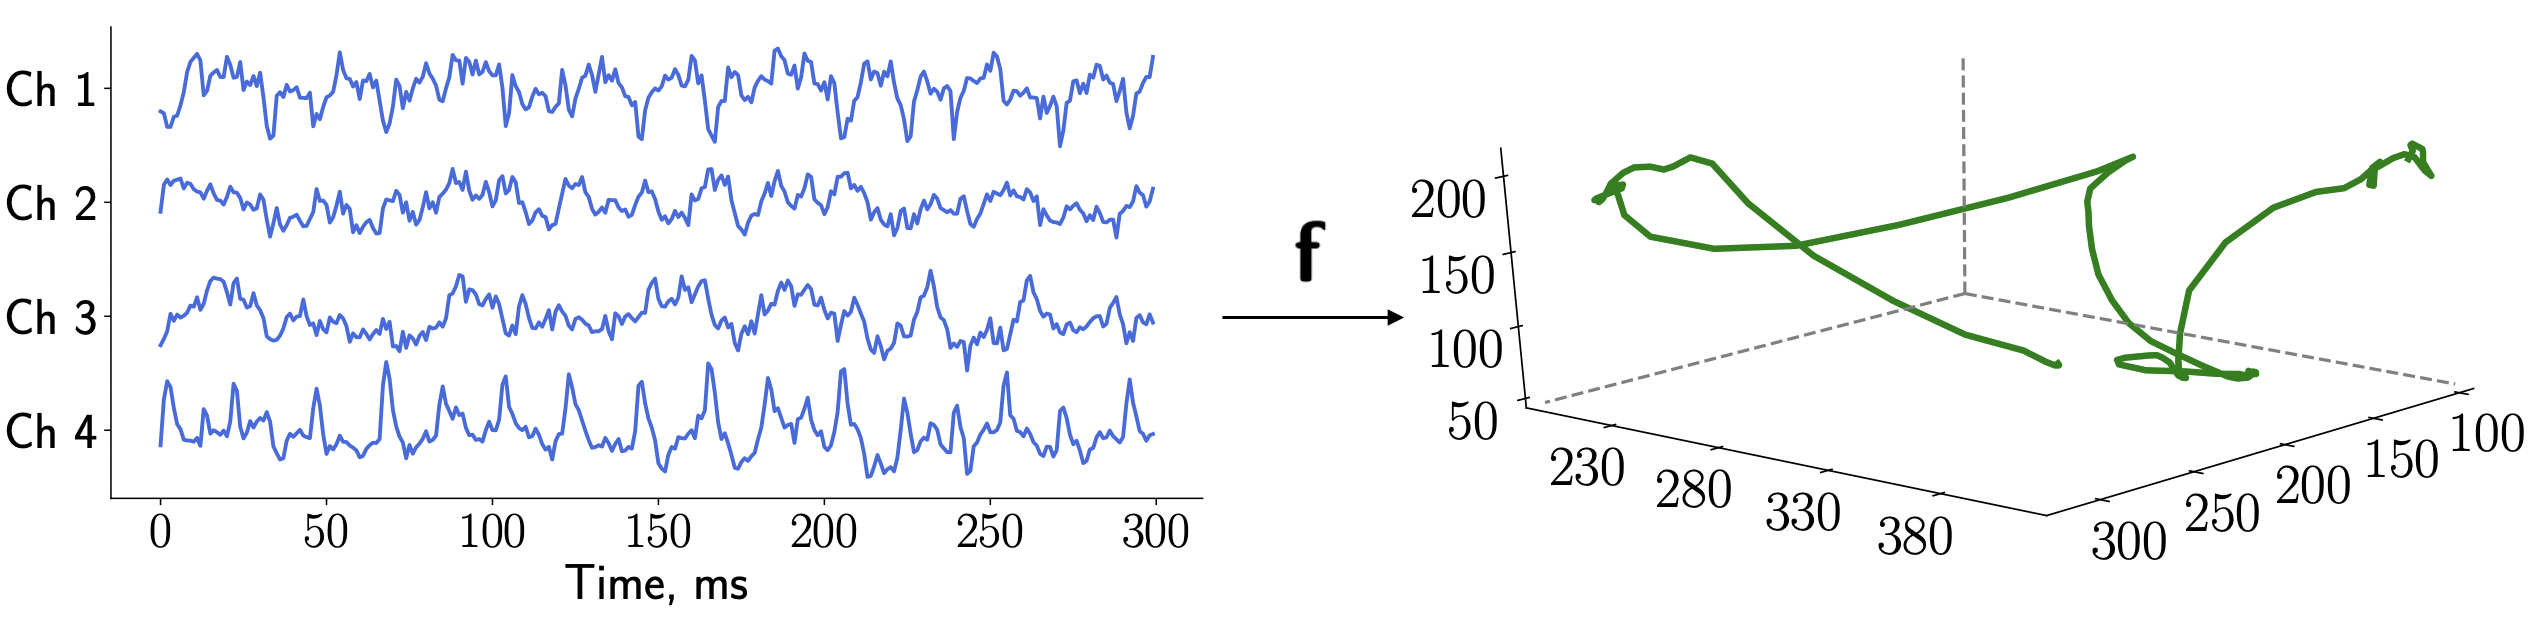
\includegraphics[width=\linewidth]{figs/slide3_1}
    \end{figure}
    \vspace{-0.15cm}
	\begin{minipage}{.48\linewidth}
		\vspace{-0.3cm}
		\begin{block}{Forecasting decoding model}
			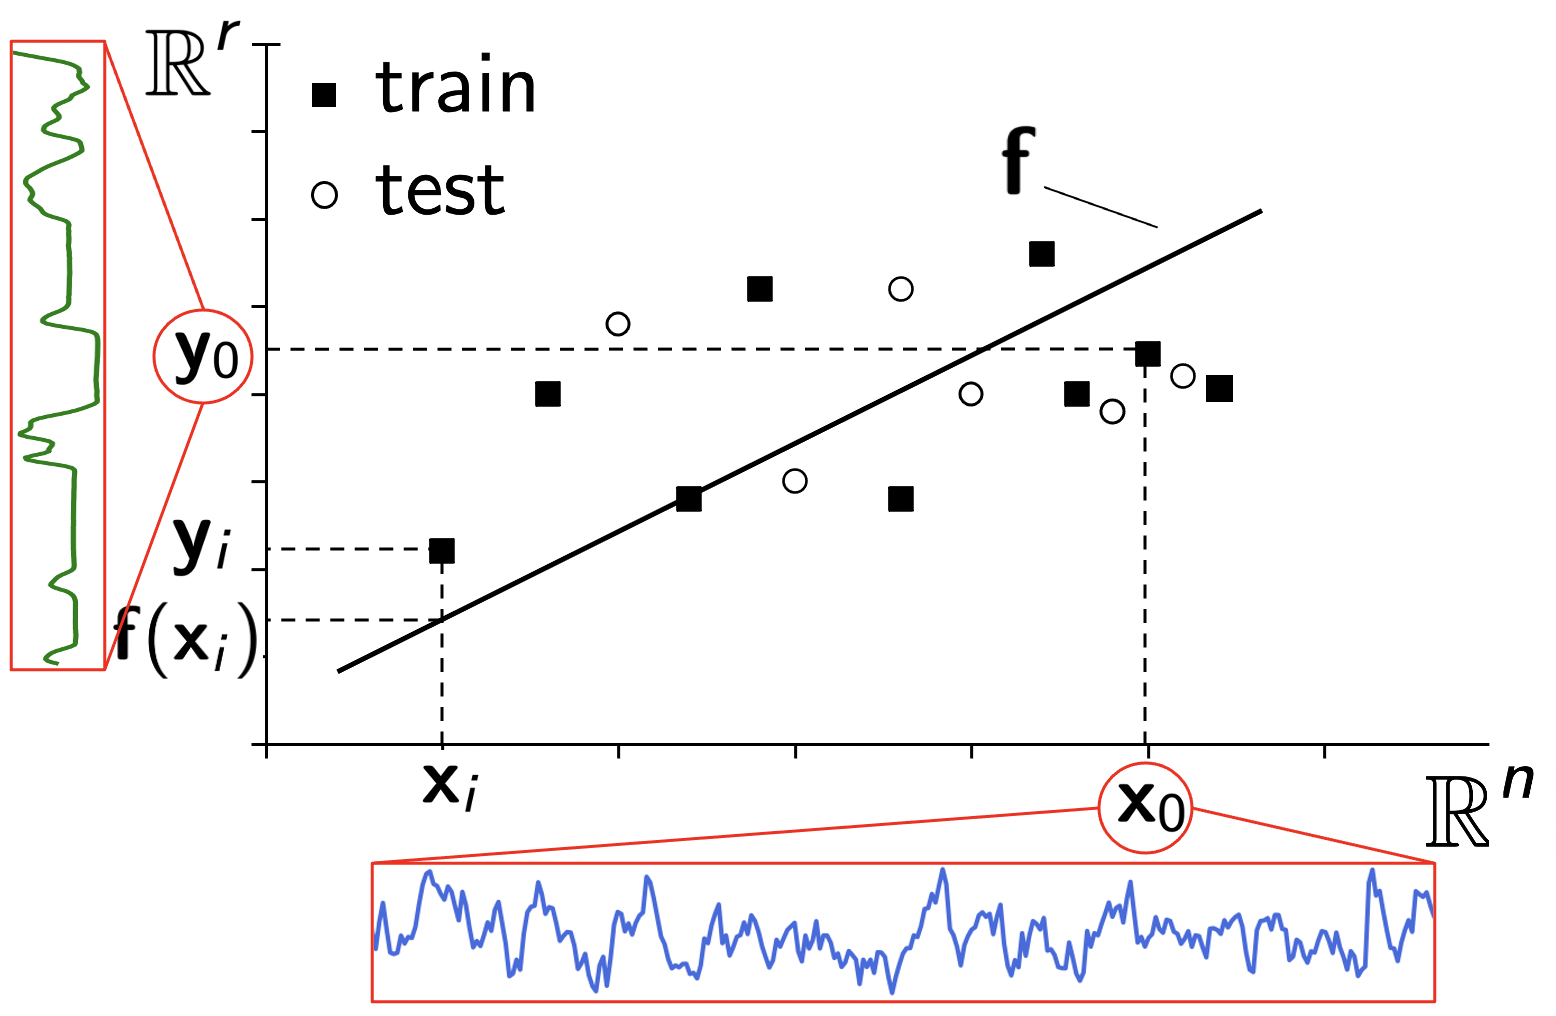
\includegraphics[width=\linewidth]{figs/slide3_3}
		\end{block}
	\end{minipage}%
	\begin{minipage}{.53\linewidth}
		\begin{block}{Hidden space concordance}
			\vspace{-0.7cm}
			\begin{equation*}
					\begin{tikzpicture}
						\matrix (m) [matrix of math nodes,row sep=2em,column sep=2em,minimum width=2em,ampersand replacement=\&]
						{
							\bx \in \bbR^n \& \& \by \in \bbR^r \\
							\& \bt, \bu \in \bbR^\ell \& \\};
						\path[-stealth]
						(m-1-1) edge node [above] {$\mathbf{f}$} (m-1-3)
						(m-1-1) edge [bend right=10] node [below, pos=0.3] {$\bW$} (m-2-2)
						(m-2-2) edge [bend right=10] node [above, pos=0.3] {$\bP$} (m-1-1)
						(m-1-3) edge [bend left=10] node [below, pos=0.3] {$\bC$} (m-2-2)
						(m-2-2) edge [bend left=10] node [above, pos=0.3] {$\bQ$} (m-1-3);
					\end{tikzpicture}
			\end{equation*}
			\vspace{-1.3cm}
			\begin{align*}
				\bx &= \bP \bt + \be_{\bx} \\
				\by &= \bQ \bu + \be_{\by} \\
			\end{align*}
			\vspace{-1.2cm}
			\[
				\text{cov} (\bt, \bu) \rightarrow \max_{\bP, \bQ}
			\]
		\end{block}
	\end{minipage}
\end{frame}
%--------------------------------------------------------------------------------
\begin{frame}{Signal decoding task}
	$\bY = \bF(\bX, \bTheta) + \bE_{\by} = \bX \cdot \bTheta^{\T}  + \bE_{\by}$ is a parametric model $\bTheta \in \bbR^{r \times n}$.
	\begin{block}{Decoding loss function}
		\vspace{-0.3cm}
		\[
			\mathcal{L}(f, \bX, \bY) = {\left\| \bY  - \bF(\bX, \bTheta) \right\| }_2^2 =  {\left\| \underset{m \times r}{\mathbf{Y}}  - \underset{m \times n}{\bX} \cdot \underset{r \times n}{\bTheta}^{\T} \right\| }_2^2 \rightarrow\min_{\bTheta}.
		\]
		\vspace{-0.3cm}
	\end{block}
	
	\begin{minipage}{0.65\linewidth}
		\begin{block}{Projection to latent space}
		\vspace{-0.7cm}
		\begin{align*}
			\bX	&= \bT \bP^{\T} + \bE_{\bx},\\
			\bY &= \bU \bQ^{\T} + \bE_{\by}.
		\end{align*}
			\end{block}
	\end{minipage}%
	\begin{minipage}{0.35\linewidth}
			\vspace{-0.1cm}
			\begin{equation*}
				\begin{tikzpicture}
					\matrix (m) [matrix of math nodes,row sep=2em,column sep=4em,minimum width=2em,ampersand replacement=\&]
					{
						\bbX \subset \bbR^n \& \bbY \subset \bbR^r \\
						\bbT \subset \bbR^\ell \& \bbU \subset \bbR^s \\};
					\path[-stealth]
					(m-1-1) edge [black] node [black, above] {$\mathbf{f}$} (m-1-2)
					(m-1-1) edge [black, bend right=10] node [black, left] {$\bW$} (m-2-1)
					(m-2-1) edge [black, bend right=10] node [black, right] {$\bP$} (m-1-1)
					(m-1-2) edge [black, bend left=10] node [black, right] {$\bC$} (m-2-2)
					(m-2-2) edge [black, bend left=10] node [black, left] {$\bQ$} (m-1-2)
					(m-2-1) edge [black] node [black, above] {$\bB$} (m-2-2);
				\end{tikzpicture}
			\end{equation*}
	\end{minipage}
	\vspace{-0.4cm}
	\begin{block}{Projection concordance}
		Link function couples images of input and target signals in latent space:
		\vspace{-0.3cm}
		\[
			\bU = \bT \bB, \quad \bB = \text{diag}(\beta_k), \quad \beta_k = \bu_k^{\T}\bt_k / (\bt_k^{\T}\bt_k).
		\]
		Decoding model:
		\vspace{-0.3cm}
		\[
			\bY = \bU \bQ^{\T} + \bE_{\by} \approx \bT \bB \bQ^{\T}+ \bE_{\by} = \bX \bW^* \bB \bQ^{\T} + \bE = \bX \bTheta^{\T} + \bE_{\by},
		\]
		\[
			\bT = \bX \bW^*, \quad \text{где \,} \bW^* = \bW (\bP^{\T} \bW)^{-1}.
		\]
	\end{block}
	 
\end{frame}
%--------------------------------------------------------------------------------
\begin{frame}{Concordance process in signal decoding task}
	The dimensionality of input and target spaces are highly redundant.
	We suggest to find manifolds of low dimensionality:
	\vspace{-0.2cm}
	\begin{equation*}
		\begin{tikzpicture}
			\matrix (m) [matrix of math nodes,row sep=2em,column sep=4em,minimum width=2em,ampersand replacement=\&]
			{
				\bbX \subset \bbR^n \& \bbY \subset \bbR^r \\
				\bbT \subset \bbR^\ell \& \bbU \subset \bbR^s \\};
			\path[-stealth]
			(m-1-1) edge [black] node [black, above] {$\mathbf{f}$} (m-1-2)
			(m-2-1) edge [black, bend right=10] node [black, right] {$\bphi_d$} (m-1-1)
			(m-2-2) edge [black, bend left=10] node [black, left] {$\bpsi_d$} (m-1-2)
			(m-1-1) edge [black, bend right=10] node [black, left] {$\bphi_e$} (m-2-1)
			(m-1-2) edge [black, bend left=10] node [black, right] {$\bpsi_e$} (m-2-2)
			(m-2-1) edge [black] node [black, above] {$\mathbf{h}$} (m-2-2);
		\end{tikzpicture}
	\end{equation*}
	$\bbT \subset \bbR^\ell$ и $\bbU \subset \bbR^s$ are \textit{latent spaces} for $\bbX \in \bbR^n$ ($\ell \leq n$) and $\bbY \in \bbR^r (s \leq r)$, if there is \textit{encoding function} $\bphi_e: \bbX \to \bbT$, $\bpsi_e: \bbY \to \bbU$ and \textit{decoding function} $\bphi_d: \bbT  \to \bbX$, $\bpsi_d: \bbU  \to \bbY$:
	\begin{align*}
	\text{for each } \bx \in \bbX &\quad \text{exists } \bt \in \bbT: \bphi_d \bigl(\bphi_e(\bx)\bigr) = \bphi_d(\bt) = \bx; \\
	\text{for each } \by \in \bbY &\quad  \text{exists } \bu \in \bbU: \bpsi_d \bigl(\bpsi_e(\by)\bigr) = \bpsi_d(\bu) = \by.
	\end{align*}

	The latent spaces $\bbT$ и $\bbU$ are called \textbf{concordant}, if there is \textit{a link function} $\mathbf{h}: \bbT \rightarrow \bbU$:
	\vspace{-0.3cm}
	\[
		\by = \mathbf{f}(\bx) = \bpsi_d\Bigl(\mathbf{h}\bigl(\bphi_e(\bx)\bigr)\Bigr).
	 \]
	 \vspace{-0.5cm}
	 \begin{block}{Projection concordance function}
	 	\vspace{-0.3cm}
	 	\[
	 		g: \bbT \times \bbU \rightarrow \bbR, \quad g(\bt, \bu) = g(\bphi_e(\bx), \bpsi_e(\by)) \rightarrow \max_{\bphi_e, \bpsi_e, \bh}
	 	\]
	 	\vspace{-0.3cm}
	 \end{block}

\end{frame}
%--------------------------------------------------------------------------------
\begin{frame}{Latent space concordant function}
	\begin{statement}[Isachenko, 2017]
		Vectors $\bt_k$ и $\bu_k$ obtained by the iterative procedure:
		\vspace{-0.2cm}
		\begin{align*}
			\bt_k &:= \frac{\bX_k \bw_k}{\|\bw_k\|}, \quad  \bw_k := \bX_k^{\T} \bu_{k-1} / (\bu_{k-1}^{\T} \bu_{k-1}); \\ 
			\bu_k &:= \frac{\bY_k \bc_k}{\| \bc_k \|}, \quad \bc_k := \bY_k^{\T} \bt_k / (\bt_k^{\T} \bt_k).
		\end{align*}
		\vspace{-0.5cm} \\
		have largest covariance $\textnormal{cov}(\bt, \bu)$.
	\end{statement}

	\begin{theorem}[Isachenko, 2017]
		In the case of a linear encoding function $\bphi_e (\bT) = \bT \bP^{\T}$, a linear decoding function $\bpsi_e (\bU) = \bU \bQ^{\T}$ and a concordance function $g(\bt, \bu) = \textnormal{cov}(\bt, \bu)$ the model parameters
		\[
		\bTheta = \bW (\bP^{\T} \bW)^{-1} \bB \bQ^{\T}
		\]
		are optimal for the model $\bF(\bX, \bTheta)$.
	\end{theorem}
\end{frame}
%--------------------------------------------------------------------------------
\begin{frame}{Example of hidden space concordant projection}
	The input variables $\bx_i \sim \mathcal{N}(0, \mathbf{\Sigma})$. \\ 
	The target variables $\by_i$ linearly depend on $pc_2$ и does not depend on $pc_1$.
	\begin{figure}[h]
	\centering
	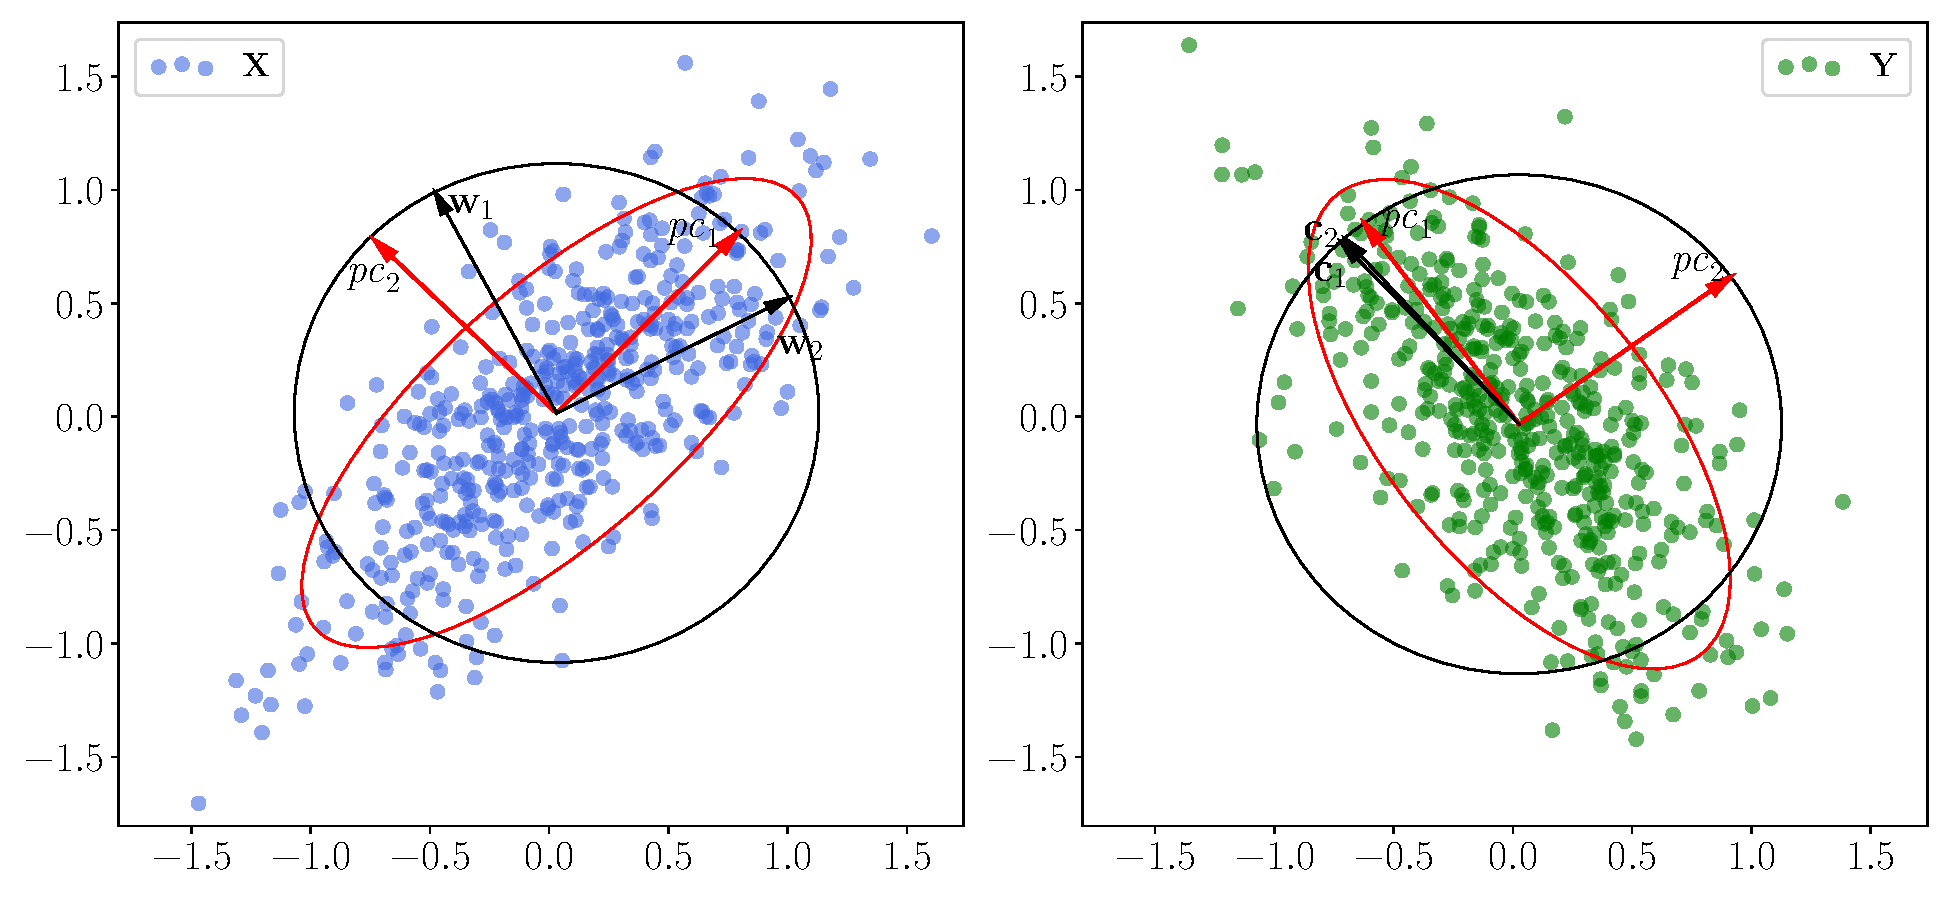
\includegraphics[width=\linewidth]{figs/pls_toy_example}
	\end{figure}
	Projection concordance of matrices~$\bX$ and~$\bY$ find optimal hidden representation, deviating vectors~$\bw_k$ and~$\bc_k$ from principal components. 
\end{frame}
%--------------------------------------------------------------------------------
\begin{frame}{Superposition of signal decoding models}
	Let $\mathbf{f}_1(\bx_1, \bTheta_1)$, $\mathbf{f}_2(\bx_2, \bTheta_2)$ be linear signal decoding models
	\begin{statement}[isachenko, 2021]
		If the decoding model is an additive superposition of linear models:
		\vspace{-0.3cm}
		\[
			\by = \mathbf{f}_1(\bx_1, \bTheta_1) + \mathbf{f}_2(\bx_2, \bTheta_2) + \boldsymbol{\varepsilon}_{\by} = \bTheta_1 \bx_1 + \bTheta_2 \bx_2 + \boldsymbol{\varepsilon}_{\by},
		\]
		then the optimal parameters are
		\vspace{-0.2cm}
		\begin{align*}
			\bTheta_1 &= (\bX_1^{\T} \bM_{\bX_2} \bX_1)^{-1} \bX_1^{\T} \bM_{\bX_2} \bY, \\
			\bTheta_2 &= (\bX_2^{\T} \bM_{\bX_1} \bX_2)^{-1} \bX_2^{\T} \bM_{\bX_1} \bY,
		\end{align*}
		where \, $\bM_{\bX_1} = \bI - \bX_1 (\bX_1^{\T} \bX_1)^{-1} \bX_1^{\T}$, \, $\bM_{\bX_2} = \bI -\bX_2 (\bX_2^{\T} \bX_2)^{-1} \bX_2^{\T}$.
	\end{statement}
	\begin{theorem}[Isachenko, 2021]
		If $\text{span}(\bX_1) \neq \text{span}(\bX_2)$, then the error of the additive superposition of linear decoding models is less or equal the error of each of the models:
		\begin{align*}
			\mathcal{L}_{\textnormal{sup}}(\bTheta_1^*, \bTheta_2^*, \bX_1, \bX_2, \bY) &\leq \mathcal{L}(\bTheta_1, \bX_1, \bY), \\
			\mathcal{L}_{\textnormal{sup}}(\bTheta_1^*, \bTheta_2^*, \bX_1, \bX_2, \bY) &\leq \mathcal{L}(\bTheta_2, \bX_2, \bY).
		\end{align*}
	\end{theorem}
\end{frame}
%--------------------------------------------------------------------------------
\begin{frame}{Nonlinear methods of hidden space concordance}
	Let encoding and decoding functions be deep neural networks:
	\vspace{-0.1cm}
	\begin{align*}
		\bT &= \bphi_e(\bX) =  \bW_x^L \sigma(\dots \sigma(\bW_x^2 \sigma(\bX \bW_x^1)) \dots ) \\
		\bU &= \bpsi_e(\bY) =  \bW_y^L \sigma(\dots \sigma(\bW_y^2 \sigma(\bY \bW_y^1)) \dots ) \\
		\bX &= \bphi_d(\bT) =  \bW_t^L \sigma(\dots \sigma(\bW_x^2 \sigma(\bT \bW_t^1)) \dots ) \\
		\bY &= \bpsi_d(\bU) =  \bW_u^L \sigma(\dots \sigma(\bW_y^2 \sigma(\bU \bW_u^1)) \dots )
	\end{align*}
	\vspace{-0.4cm}
	\begin{block}{Projection concordance}
		\vspace{-0.3cm}
		\[
			g(\bT, \bU) \rightarrow \max_{\bW}, \quad \bW = \{\bW_x^i, \bW_y^i, \bW_t^i, \bW_u^i\}_{i=1}^L.
		\]
	\end{block}	
	\vspace{-0.3cm}
		The gradient of the concordance function $g(\bt, \bu) = \textnormal{corr}(\bt, \bu)$ is
		\[
			\frac{\partial g(\bt, \bu)}{\partial \bt} = \frac{1}{\ell - 1} \left(\bSigma_1^{-1/2} \bU \bV^{\T} \bSigma_2^{-1/2} \bU - \bSigma_1^{-1/2} \bU \bD \bV^{\T} \bSigma_1^{-1/2} \right),
		\]
		where $\bU, \bD, \bV = \textnormal{SVD}(\bSigma)$, \, $\bSigma = \bSigma_1^{-1/2} \bSigma_{12} \bSigma_2^{-1/2} $, \, $\bSigma_1 = \frac{1}{\ell - 1} \bT \bT^{\T}$, \, $\bSigma_2 = \frac{1}{\ell - 1} \bU \bU^{\T}$, \, $\bSigma_{12} = \frac{1}{\ell - 1} \bT \bU^{\T}$.
\end{frame}
%--------------------------------------------------------------------------------
\begin{frame}{Feature selection for signal decoding task}
	$\bX = [\bchi_1, \dots, \bchi_n] \in \bbR^{m \times n}$ is the input variable matrix; $\bY = [\bnu_1, \dots, \bnu_r] \in \bbR^{m \times r}$ is the target variable matrix. \\
	The goal of feature selection is to find~$\ba = \{0, 1\}^n$, which components are the indicators of selected features. 
	\begin{block}{Feature selection loss function}
		\vspace{-0.3cm}
		\[
			\bz = \argmin_{\bz' \in [0, 1]^n} S(\bz', \bX, \bY), \quad 
		a_j = [z_j > \tau].
		\]
		\vspace{-0.2cm}
	\end{block}
	\begin{block}{Loss function of decoding model}
		\vspace{-0.6cm}
		\[
			\mathcal{L}(\bTheta_{\ba}, \bX_{\ba}, \bY) = {\left\| \mathbf{Y} - \bX_{\ba}\bTheta^{\T}_{\ba} \right\| }_2^2 \rightarrow\min_{\bTheta_{\ba}}, \quad \bX_{\ba} = \{\bchi_j: a_j = 1, \, j = 1, \dots, n\}
		\]
		\vspace{-0.6cm}
	\end{block}
	\begin{block}{Quadratic programming feature selection}
	\vspace{-0.3cm}
	\[
	S(\bz, \bX, \bnu) = (1 - \alpha) \cdot \underbrace{\bz^{\T} \bQ \bz}_{\text{Sim}(\bX)} - \alpha \cdot \underbrace{\vphantom{()} \mathbf{b}^{\T} \bz}_{\text{Rel}(\bX, \bnu)} \rightarrow \min_{\substack{\bz \geq \bZero_n \\ \bOne_n^{\T} \bz=1}}.
	\]
	\vspace{-0.5cm}
	\end{block}
		$\bz \in [0, 1]^n$ is a feature importance score; \\
		$\bQ = \bigl[\left|\text{corr}(\bchi_i, \bchi_j)\right|\bigr]_{i,j=1}^n \in \bbR^{n \times n}$ is a pairwise feature similarity matrix; \\
		$\mathbf{b} = \bigl[\left|\text{corr}(\bchi_i, \bnu)\right|\bigr]_{i=1}^n \in \bbR^n$ is a vector of feature relevancies. 
\end{frame}
%--------------------------------------------------------------------------------
\begin{frame}{Quadratic programming feature selection}
		\[
		S(\bz, \bX, \bnu) = (1 - \alpha) \cdot \underbrace{\bz^{\T} \bQ \bz}_{\text{Sim}(\bX)} - \alpha \cdot \underbrace{\vphantom{()} \mathbf{b}^{\T} \bz}_{\text{Rel}(\bX, \bnu)} \rightarrow \min_{\substack{\bz \geq \bZero_n \\ \bOne_n^{\T} \bz=1}}.
		\]

	\begin{theorem}[Isachenko, 2018]
		Let the pairwise feature similarity matrix~$\hat{\bQ}$ is obtained by semidefinite relaxation of initial matrix~$\bQ$:
		\vspace{-0.2cm}
		\begin{equation*}
			\hat{\bQ} = \bQ - \lambda_{\min}(\bQ) \bI.
		\end{equation*}
		\vspace{-0.7cm} \\
		Then quadratic programming feature selection task has a unique global minimum.
	\end{theorem}
	\begin{block}{Relevance agregation (RelAgg)}
	\vspace{-0.2cm}
		\[
			\bb = \bigl[\left|\text{corr}(\bchi_i, \bnu)\right|\bigr]_{i=1}^n \rightarrow \bb = \left[\sum_{k=1}^r\left|\text{corr}(\bchi_i, \bnu_k)\right|\right]_{i=1}^n.
		\]
	\end{block}
	{\bf Drawback:} dependencies in the target space of the matrix~$\bY$ are not taking into account. 
	
\end{frame}
%--------------------------------------------------------------------------------
\begin{frame}{Feature selection in signal decoding task}
	\begin{block}{Symmetric Importance (SymImp)}
	Let penalize target vectors by introducing the term~$\text{Sim} (\bY)$:
	\[
	S(\bz, \bX, \bY) = \alpha_1 \cdot \underbrace{\bz_x^{\T} \bQ_x \bz_x}_{\text{Sim}(\bX)} - \alpha_2 \cdot \underbrace{\bz_x^{\T} \bB \bz_y}_{\text{Rel}(\bX, \bY)} + \alpha_3 \cdot \underbrace{\bz_y^{\T} \bQ_y \bz_y}_{\text{Sim}(\bY)} \rightarrow \min_{\substack{\bz_x \geq \bZero_n, \, \bOne_n^{\T}\bz_x=1 \\ \bz_y \geq \bZero_r, \, \bOne_r^{\T}\bz_y=1}},
	\]
	\[
	\bQ_x = \bigl[ \left| \text{corr}(\bchi_i, \bchi_j) \right| \bigr]_{i,j=1}^n, \,
	\bQ_y = \bigl[ \left| \text{corr}(\bnu_i, \bnu_j) \right| \bigr]_{i,j=1}^r, \,
	\bB =  \bigl[ \left| \text{corr}(\bchi_i, \bnu_j) \right| \bigr]_{\substack{i=1, \dots, n \\ j=1, \dots, r}},
	\]
	\[
	\alpha_1 + \alpha_2 + \alpha_3 = 1, \quad \alpha_i \geq 0.
	\] 
	\end{block}
	SymImp penalizes correlated target vectors, which are less explained by features.
		
	\begin{block}{Assymetric Importance (AsymImp)}
		\vspace{-0.2cm}
		\begin{equation*}
		\alpha_1 \cdot \underbrace{\bz_x^{\T} \bQ_x \bz_x}_{\text{Sim}(\bX)} - \alpha_2 \cdot  \underbrace{\left(\bz_x^{\T} \bB \bz_y - \bb^{\T} \bz_y \right) }_{\text{Rel}(\bX, \bY)} + \alpha_3 \cdot \underbrace{\bz_y^{\T} \bQ_y \bz_y}_{\text{Sim}(\bY)} \rightarrow \min_{\substack{\bz_x \geq \bZero_n, \, \bOne_n^{\T}\bz_x=1 \\ \bz_y \geq \bZero_r, \, \bOne_r^{\T}\bz_y=1}}.
		\end{equation*}
		\vspace{-0.4cm} \\
		In the case of $b_j = \max\limits_{i=1, \dots n} [\bB]_{i, j}$ the components of~$\bz_y$ in~$\text{Rel}(\bX, \bY)$ are non-negative.
	\end{block}
\end{frame}
%--------------------------------------------------------------------------------
\begin{frame}{Feature selection in signal decoding task}
	\[
		\alpha_1 \cdot \underbrace{\bz_x^{\T} \bQ_x \bz_x}_{\text{Sim}(\bX)} - \alpha_2 \cdot \underbrace{\vphantom{()} \bz_x^{\T}\mathbf{B} \bz_y}_{\text{Rel}(\bX, \bY)} \rightarrow \min_{\substack{\bz_x \geq \bZero_n \\ \bOne_n^{\T}\bz_x=1}}; \quad
		\alpha_3 \cdot \underbrace{\bz_y^{\T} \bQ_y \bz_y}_{\text{Sim}(\bY)} + \alpha_2 \cdot \underbrace{\vphantom{()} \bz_x^{\T} \mathbf{B} \bz_y}_{\text{Rel}(\bX, \bY)} \rightarrow \min_{\substack{\bz_y \geq \bZero_r  \\ \bOne_r^{\T}\bz_y=1}}.
	\]
	\vspace{-0.3cm}
	\begin{block}{MinMax or MaxMin}
		\vspace{-0.6cm}
		\[
		S(\bz, \bX, \bY) = \min_{\substack{\bz_x \geq \bZero_n \\ \bOne_n^{\T}\bz_x=1}} 	\max_{\substack{\bz_y \geq \bZero_r \\ \bOne_r^{\T}\bz_y=1}} \Bigl(\text {or} \, \max_{\substack{\bz_y \geq \bZero_r \\ \bOne_r^{\T}\bz_y=1}} \min_{\substack{\bz_x \geq \bZero_n \\ \bOne_n^{\T}\bz_x=1}}\Bigr) \Bigl[\alpha_1 \cdot \underbrace{\bz_x^{\T} \bQ_x \bz_x}_{\text{Sim}(\bX)} - \alpha_2 \cdot \underbrace{\bz_x^{\T} \bB \bz_y}_{\text{Rel}(\bX, \bY)} - \alpha_3 \cdot \underbrace{\bz_y^{\T} \bQ_y \bz_y}_{\text{Sim}(\bY)}\Bigr].
		\]
	\end{block}
	\vspace{-0.4cm}
	\begin{theorem}[Isachenko, 2018]
		In the case of positive definite matrices $\bQ_x$ and $\bQ_y$, minmax and maxmin problems have the same value of the loss function $S(\bz, \bX, \bY)$
	\end{theorem}
	\vspace{-0.2cm}
	\begin{theorem}[Isachenko, 2018]
		Minmax task is equivalent to the quadratic programming task with $n + r + 1$ variables.
	\end{theorem}
	Semidefinite relaxation by shifting the matrix spectrum makes the task convex.

\end{frame}
%--------------------------------------------------------------------------------
\begin{frame}{Generalization of the proposed feature selection methods}
	\begin{theorem}[Isachenko, 2018]
		In the case of the scalar target variable $r=1$, the proposed feature selection methods (SymImp, MinMax, MaxMin, AsymImp) coincide with the original problem of minimizing the loss function $S(\bz, \bX, \bY)$.
	\end{theorem}
	\begin{table}
		\centering
		\footnotesize{
			\begin{tabular}{c|c|c}
				\hline
				Method & Criterion & Loss function $S(\bz, \bX, \bY)$ \\
				\hline && \\ 
				RelAgg & $\min \bigl[ \text{Sim}(\bX) - \text{Rel}(\bX, \bY) \bigr] $ & $\min\limits_{\bz_x} \bigl[ (1 - \alpha) \cdot \bz_x^{\T} \bQ_x \bz_x - \alpha \cdot \bz_x^{\T} \bB \bOne_r \bigr] $ \\ &&\\
				SymImp & $\begin{aligned} \min \, \bigl[ \text{Sim}(\bX) & - \text{Rel}(\bX, \bY) \\ & + \text{Sim}(\bY) \bigr] \end{aligned}$ & $ \min\limits_{\bz_x, \, \bz_y} \left[ \alpha_1 \cdot \bz_x^{\T} \bQ_x \bz_x - \alpha_2 \cdot \bz_x^{\T} \bB \bz_y + \alpha_3 \cdot \bz_y^{\T} \bQ_y \bz_y \right] $\\ &&\\ 
				MinMax & $\begin{aligned} &\min \, \bigl[ \text{Sim}(\bX) - \text{Rel}(\bX, \bY) \bigr]  \\ & \max \bigl[\text{Rel}(\bX, \bY) + \text{Sim}(\bY) \bigr] \end{aligned}$ & $	\min\limits_{\bz_x} 	\max\limits_{\bz_y} \bigl[\alpha_1 \cdot \bz_x^{\T} \bQ_x \bz_x - \alpha_2 \cdot \bz_x^{\T} \bB \bz_y - \alpha_3 \cdot \bz_y^{\T} \bQ_y \bz_y \bigr]$ \\ &&\\ 
				AsymImp & $\begin{aligned} & \min \, \bigl[ \text{Sim}(\bX) - \text{Rel}(\bX, \bY) \bigr]\\ &  \max \bigl[\text{Rel}(\bX, \bY) + \text{Sim}(\bY) \bigr] \end{aligned}$ & $\min\limits_{\bz_x, \bz_y} \bigl[ \alpha_1 \bz_x^{\T} \bQ_x \bz_x - \alpha_2 \left(\bz_x^{\T} \bB \bz_y - \bb^{\T} \bz_y \right) + \alpha_3  \bz_y^{\T} \bQ_y \bz_y \bigr]$\\  && \\
				\hline
		\end{tabular}}
	\end{table}
\end{frame}
%--------------------------------------------------------------------------------
\begin{frame}{Optimization of nonlinear models using quadratic programming}
	Let call the parameter $\theta_j$ of the model $f(\bx, \btheta)$ \textbf{active}, if $\bJ^{\T} (\mathbf{f}(\bx, \btheta) - \by) \neq 0$.
	\begin{theorem}[Isachenko, 2018]
		For differentiable model $\mathbf{f}(\bx, \btheta)$ the problem of selecting the model active parameters by the quadratic programming in the case of Newton method takes the form:
		
		\begin{minipage}{0.55\linewidth}
				\[
				S(\bz, \bX, \bnu) = (1 - \alpha) \cdot \underbrace{\bz^{\T} \bQ \bz}_{\textnormal{Sim}(\bJ)} - \alpha \cdot \underbrace{\vphantom{()} \mathbf{b}^{\T} \bz}_{\textnormal{Rel}(\bJ,  \mathbf{f} - \by)} \rightarrow \min_{\substack{\bz \geq \bZero_n \\ \bOne_n^{\T} \bz=1}},
				\]
			where
			\begin{equation*}
				 \bJ = 
				\begin{pmatrix}
					\frac{\partial f(\bx_1 , \btheta)}{\partial \theta_1} & \dots & 
					\frac{\partial f(\bx_1 , \btheta)}{\partial \theta_p} \\
					\dots & \dots & \dots \\
					\frac{\partial f(\bx_m , \btheta)}{\partial \theta_1} & \dots & 
					\frac{\partial f(\bx_m , \btheta)}{\partial \theta_p}
				\end{pmatrix}.
			\end{equation*}
		\end{minipage}%
		\begin{minipage}{0.45\linewidth}
			\begin{figure}
				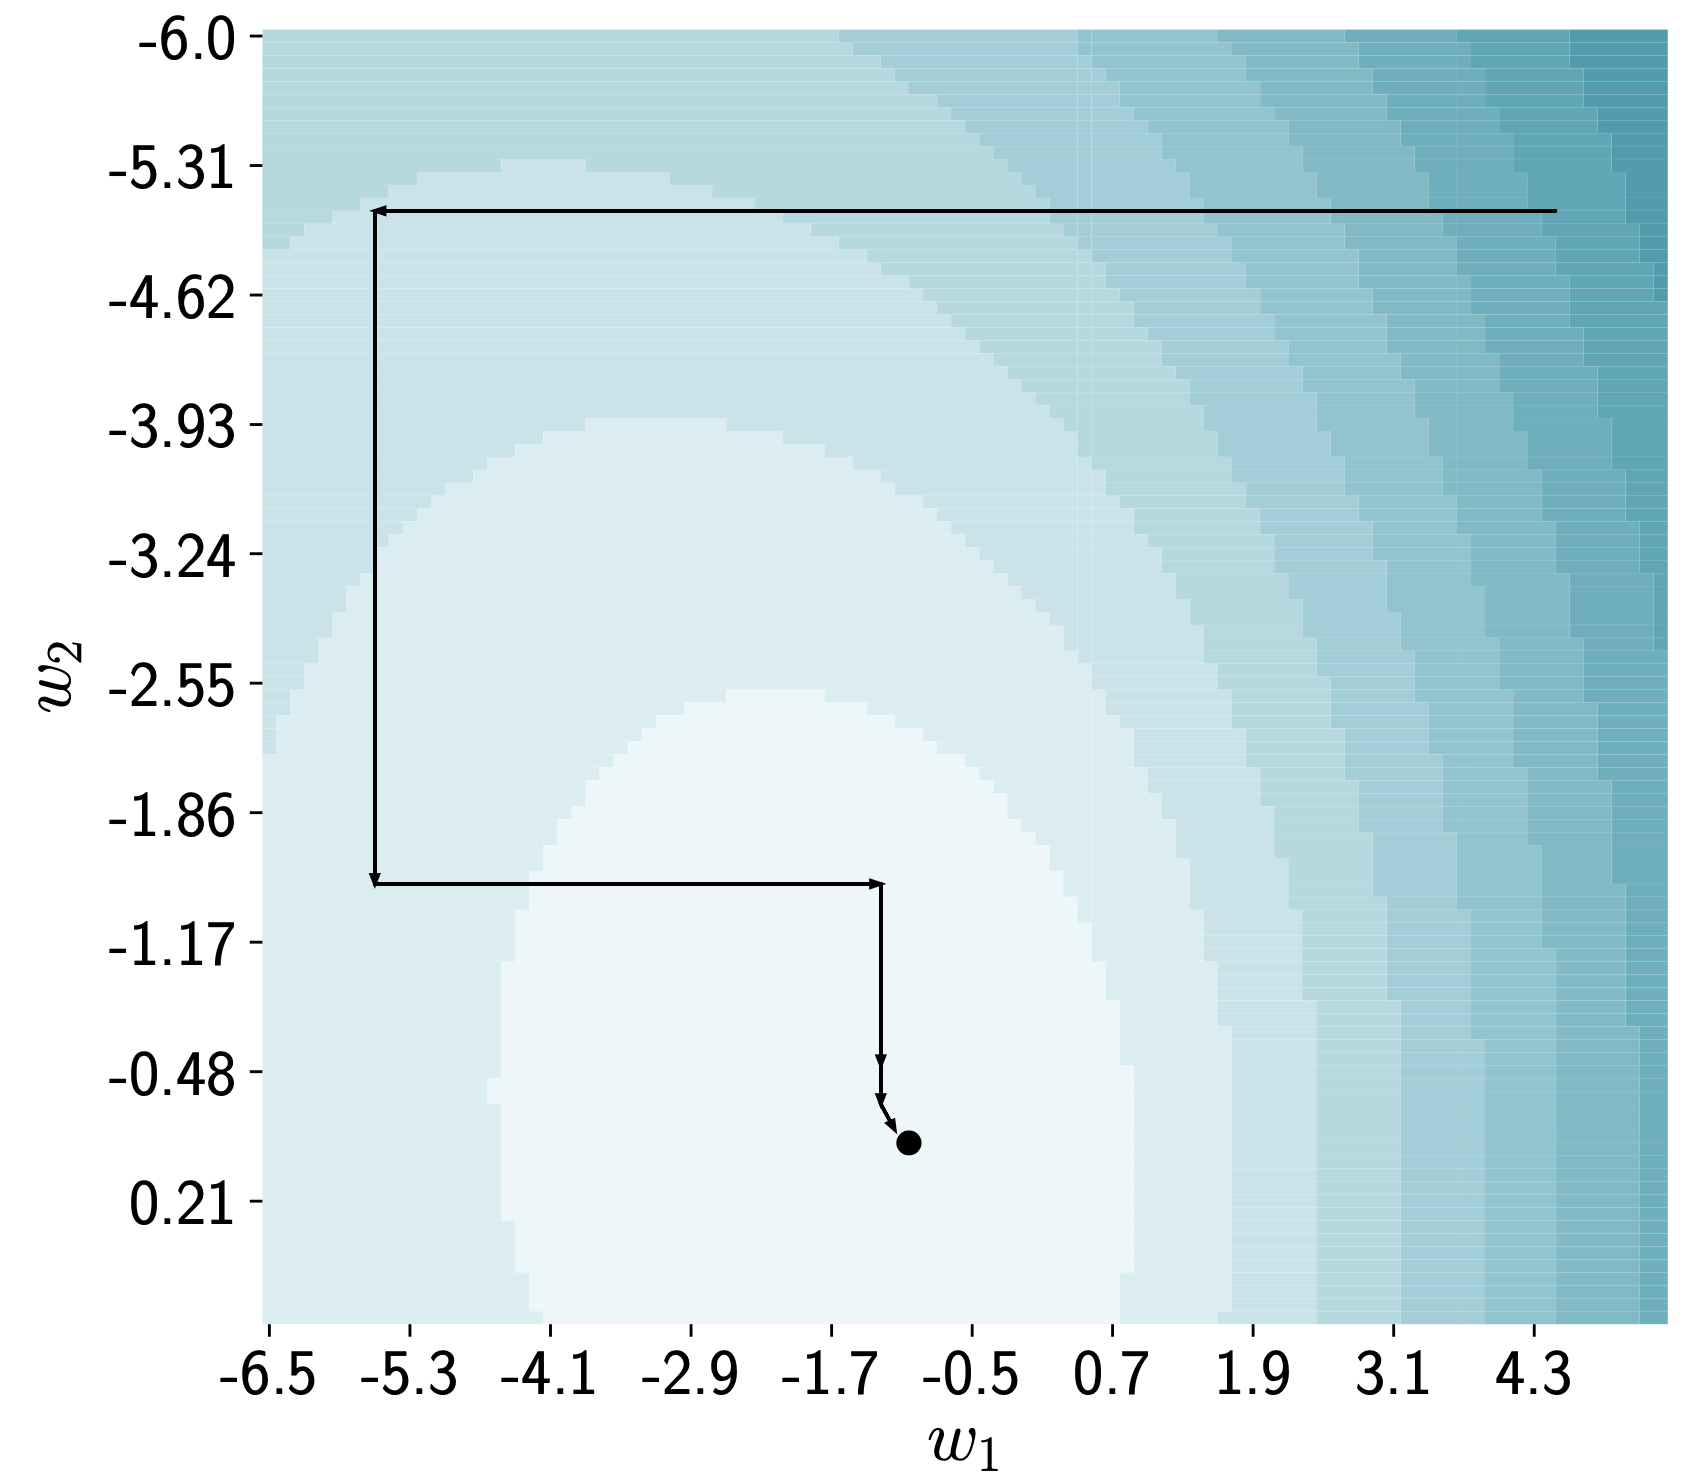
\includegraphics[width=0.9\linewidth]{figs/newton_qpfs}
			\end{figure}
		\end{minipage}
	\end{theorem}
\end{frame}
%--------------------------------------------------------------------------------
\begin{frame}{Quality criteria for solving the decoding task}

\begin{block}{Normalized RMSE}
	Forecasting quality:
	\vspace{-0.2cm}
	\[
		\text{sRMSE}(\bY, \widehat{\bY}_{\ba}) = \sqrt{\frac{\text{MSE} (\bY, \widehat{\bY}_{\ba})}{\text{MSE} (\bY, \overline{\bY})}} =  \frac{\| \bY - \widehat{\bY}_{\ba} \|_2}{\| \bY - \overline{\bY} \|_2}, \quad \text{где} \quad \widehat{\bY}_{\ba} = \bX_{\ba} \bTheta_{\ba}^{\T}.
	\]
	\vspace{-0.2cm}
	$\overline{\bY}$~--- constant forecast.
\end{block}

\begin{block}{Multicorrelation}
	The mean value of coefficient of multiple correlation:
	\vspace{-0.2cm}
	\[
		R^2 = \frac{1}{r} \text{tr} \left( \bC^{\T} \mathbf{R}^{-1} \bC \right), \quad \bC = [ \text{corr}(\bchi_i, \bnu_j)]_{\substack{i=1, \dots, n \\ j=1, \dots, r}}, \, \mathbf{R} = [ \text{corr}(\bchi_i, \bchi_j)]_{i, j = 1}^n.
	\]
\end{block}
\vspace{-0.4cm}
\begin{block}{Bayesian information criteria}
	Trade-off of forecast quality and model complexity~$\|\ba\|_0$:
	\vspace{-0.3cm}
	\[
		\text{BIC} = m \ln \left( \text{MSE} ( \bY, \widehat{\bY}_{\ba})\right) + \| \ba \|_0 \cdot \log m.
	\]
\end{block}
\end{frame}
%--------------------------------------------------------------------------------
\begin{frame}{Electrocorticogram signal decoding task}
    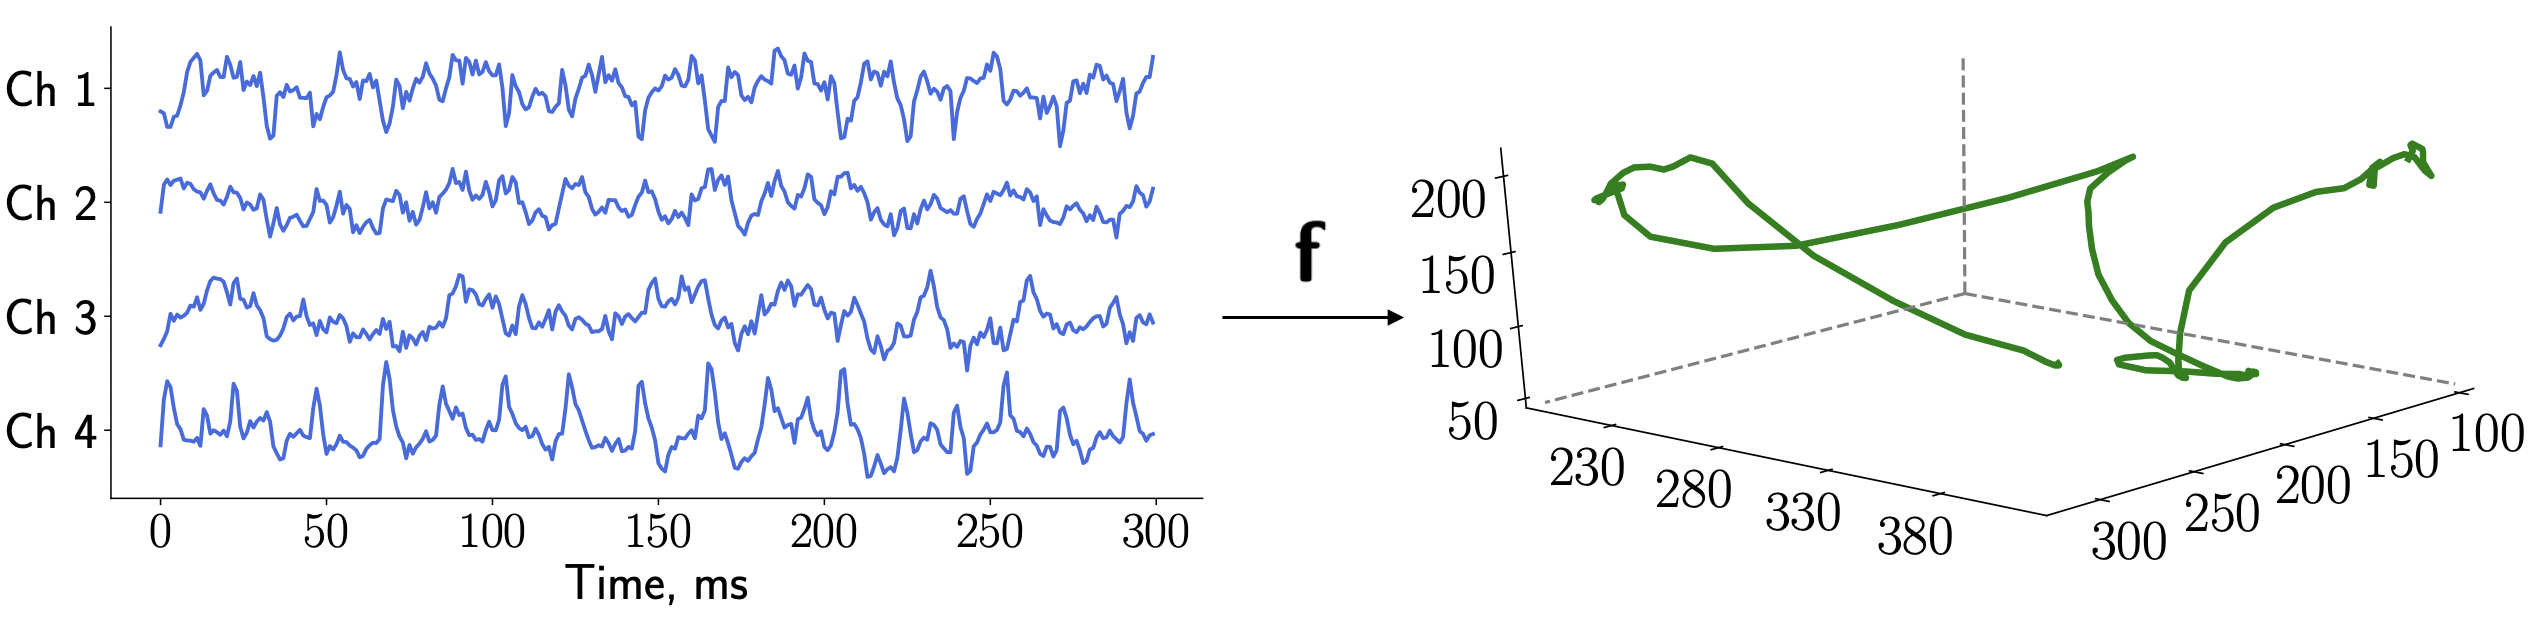
\includegraphics[width=1.0\linewidth]{figs/slide3_1}
	\begin{minipage}{.58\linewidth}
 	There are given: \\
	$\bX \in \bbR^{m \times (32 \cdot 27)}$ -- ECoG signals, \\
	$\bY \in \bbR^{m \times 3k}$ -- hand trajectory, where
	\vspace{0.1cm}
	\[
		\bY = 
		\begin{pmatrix}
		x_1 \,\, y_1 \,\, z_1 & \dots & x_{k\hphantom{+1}} \,\, y_{k\hphantom{+1}} \,\, z_{k\hphantom{+1}}\\
		x_2 \,\, y_2 \,\, z_2 & \dots & x_{k + 1} \,\, y_{k + 1} \,\, z_{k + 1}\\
		 \dots & \dots & \dots  \\
		x_m \, y_m \, z_m & \dots & x_{m + k} \, y_{m + k} \, z_{m + k}
		\end{pmatrix}.
	\]
	Columns of matrix $\bY$ are highly correlated in the time axis.
	\end{minipage}%
	\begin{minipage}{.42\linewidth}
		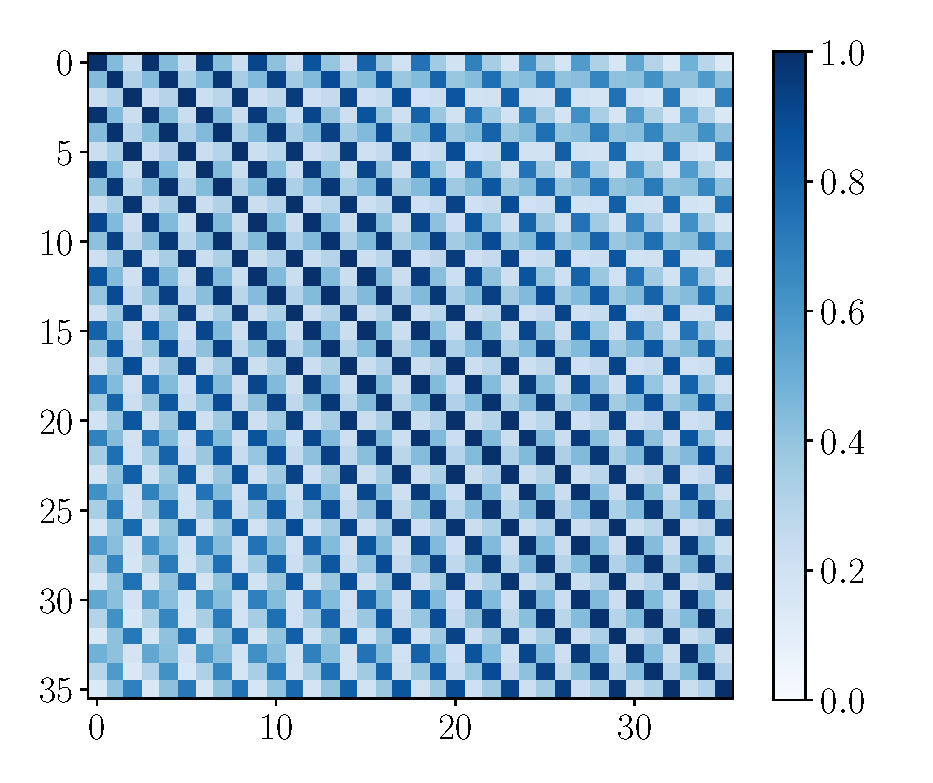
\includegraphics[width=\linewidth]{figs/Y_corr_matrix.eps} \\
		\centering Correlation matrix $\bY$
	\end{minipage}
	\\
	\url{http://neurotycho.org}
\end{frame}
%--------------------------------------------------------------------------------
\begin{frame}{Analysis of the proposed feature selection methods}
	\begin{figure}
		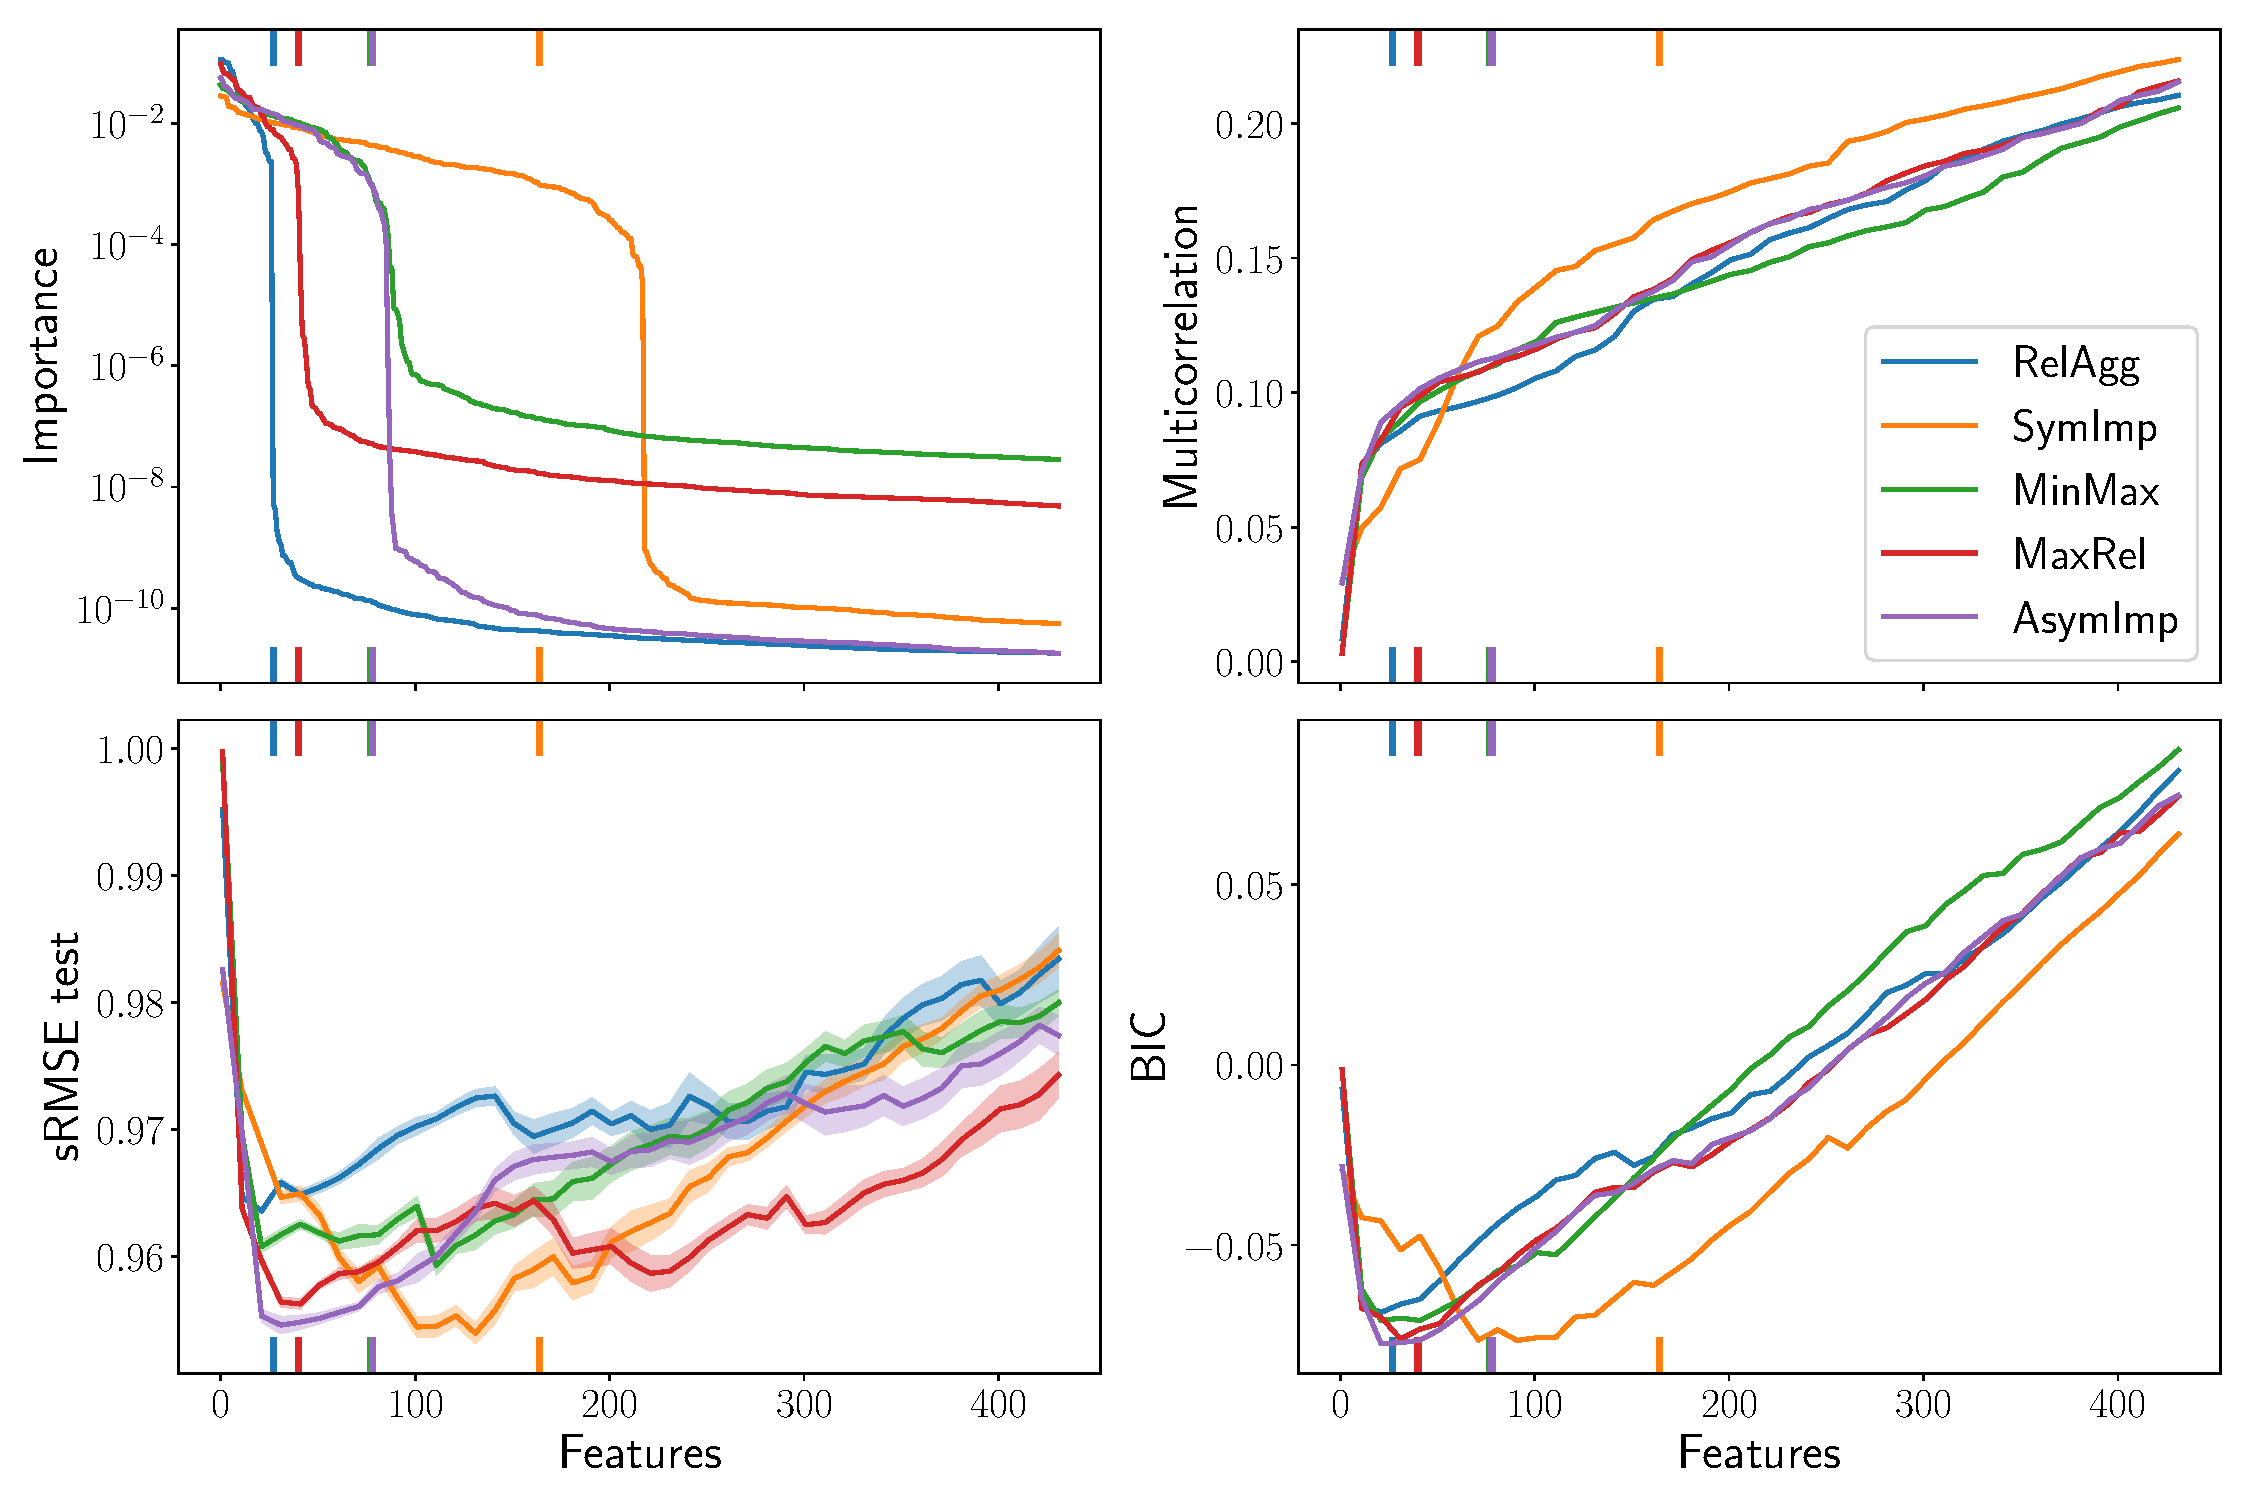
\includegraphics[width=0.9\linewidth]{figs/ecog_3_30_metrics.pdf}
		\vspace{-0.2cm}
	\end{figure}
	The proposed methods for model selection have the smaller error in relation to the basic method.
\end{frame}
%--------------------------------------------------------------------------------
\begin{frame}{Comparison of PLS method with the feature selection methods}

\begin{figure}[h]
	\begin{minipage}{.43\linewidth}
		\centering
		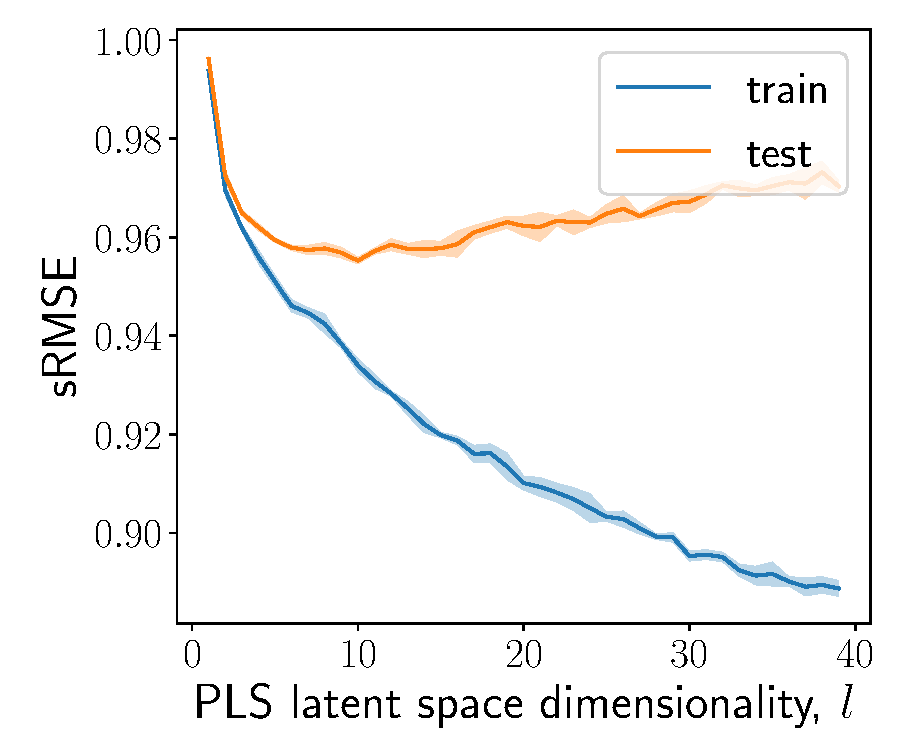
\includegraphics[width=1.\linewidth]{figs/pls_vs_k}
	\end{minipage}%
	\begin{minipage}{.57\linewidth}
		\centering
		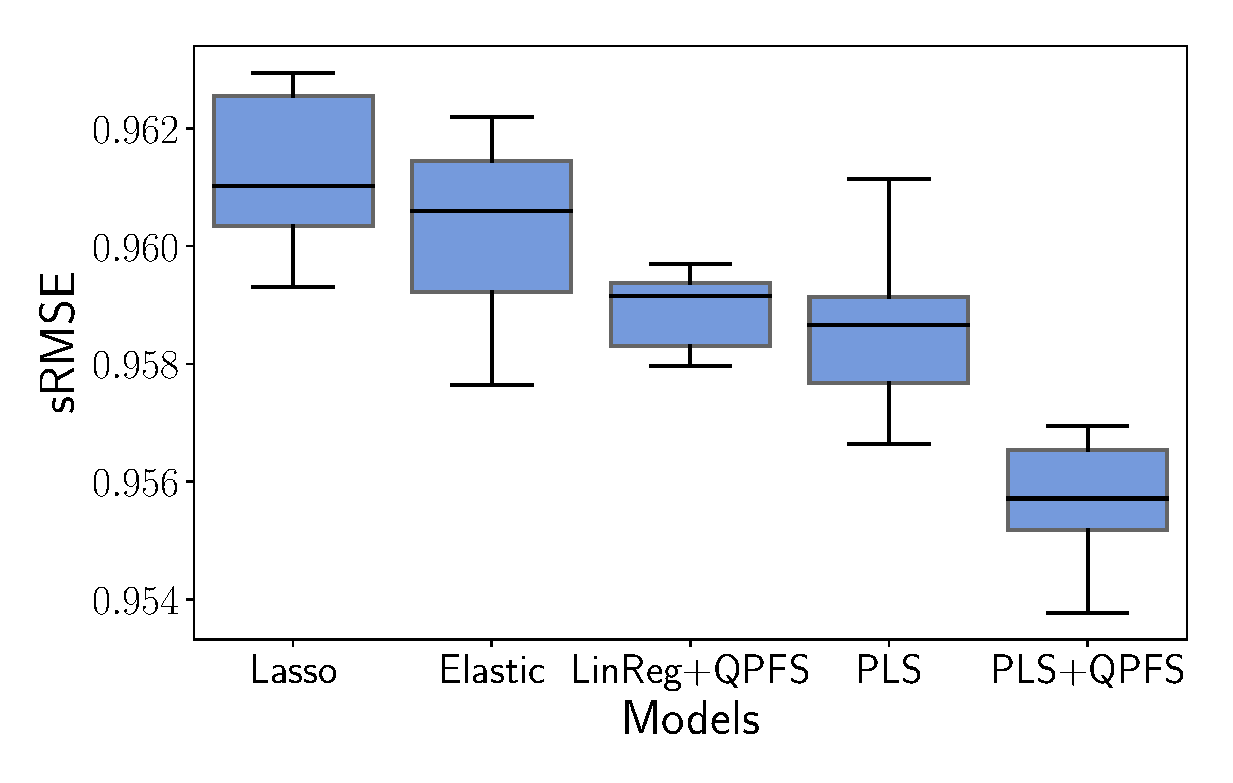
\includegraphics[width=1.\linewidth]{figs/models2}
	\end{minipage}
\end{figure}
\begin{itemize}
	\item The proposed feature selection methods achieve a lower error compared to the basic Lasso and Elastic algorithms.
	\item PLS shows comparable quality with QPFS.
	\item A combination of two methods shows the best result.
	\end{itemize}

\end{frame}
%--------------------------------------------------------------------------------
\begin{frame}{Research results}
\begin{enumerate}
	\item We have investigated the problem of the signal dimensionality reduction in highly correlated spaces.
	We have proposed signal decoding methods that take into account the dependencies both in the input and in the target signal spaces.
	\vfill
	\item We have proved the optimality theorems for the proposed methods of signal decoding. The proposed methods select consistent models in the case of excessive dimensionality of the data description.
	\vfill
	\item We have proposed feature selection methods that take into account dependencies in both the input and target spaces. The proposed methods give stable and adequate solutions in high-dimensional spaces.
	\vfill
	\item Nonlinear methods for hidden space concordance for complex structured target variable are proposed.
	\vfill
	\item We have proposed the number of forecasting models for heterogeneous sets of signals that are suitable for the task of modelling brain computer interfaces.
\end{enumerate}
\end{frame}
%--------------------------------------------------------------------------------
\begin{frame}{Publication list}
	\vspace{-0.1cm}
	\begin{block}{Papers}
		\vspace{-0.1cm}
		{\scriptsize
		\begin{enumerate}
			\item Isachenko R., Strijov V. Quadratic Programming Feature Selection for Multicorrelated Signal Decoding with Partial Least Squares \emph{Expert Systems with Applications}, 2021, на рецензировании.
			\item Исаченко Р.В., Яушев Ф.Р., Стрижов В.В. Модели согласования скрытого пространства в задаче прогнозирования // Системы и средства информатики, 31(1), 2021.
			\item Isachenko~R., Vladimirova~M., Strijov~V. Dimensionality Reduction for Time Series Decoding and Forecasting Problems. \emph{DEStech Transactions on Computer Science and Engineering}, optim, 2018.
			\item Isachenko~R., Strijov~V. Quadratic programming optimization for Newton method. \emph{Lobachevskii Journal of Mathematics}, 39(9), 2018.
			\item Isachenko~R. et al. Feature Generation for Physical Activity Classification. \emph{Artificial Intellegence and Decision Making}, 3, 2018.
			\item Исаченко Р.В., Стрижов В. В. Метрическое обучение в задачах мультиклассовой классификации временных рядов \emph{Информатика и её применения}, 10(2), 2016.
		\end{enumerate}
	}
	\end{block}
\vspace{-0.3cm}
\begin{block}{Conferences}
	\vspace{-0.1cm}
	{\scriptsize
	\begin{enumerate}
		\item  Intelligent Data Processing Conference, 2020, Снижение размерности в задаче декодирования временных рядов.
		\item  Intelligent Data Processing Conference, 2018, Dimensionality reduction for multicorrelated signal decoding with projections to latent space. 
		\item Математические методы распознавания образов, 2017. Локальные модели для классификации объектов сложной структуры.
		\item Intelligent Data Processing Conference, 2016. Multimodel forecasting multiscale time series in internet of things.
		\item Ломоносов, 2016. Метрическое обучение в задачах мультиклассовой классификации временных рядов.
	\end{enumerate}
	}
\end{block}
\end{frame}
\end{document} 
